%! Author = Omar Iskandarani
%! Date = 2/15/2025

\documentclass[a4paper, aps,preprint,superscriptaddress, 12pt]{revtex4}
\usepackage[paperwidth=210mm, paperheight=297mm, margin=2.5cm]{geometry}
\usepackage{float}
\usepackage{tikz}
\usepackage[font=footnotesize]{caption}
\usetikzlibrary{arrows.meta}
\usepackage{pgfplots}
\pgfplotsset{compat=1.18}
\usetikzlibrary{arrows.meta}
\usepackage[none]{hyphenat}
\usepackage{array}
\usepackage{amsmath, amssymb}
\usepackage{booktabs, array, multirow}
\usepackage[utf8]{inputenc}
\usepackage{amssymb}
\usepackage{graphicx}
\usepackage{hyperref}
\usepackage{physics}
\usepackage{multirow}
\usepackage{natbib}
\usepackage{url}
\renewcommand{\arraystretch}{1.5}
\renewcommand{\floatpagefraction}{.8}
\sloppy

\begin{document}
\author{Omar Iskandarani}
\title{
    Wervelingsklokken en door vorticiteit geïnduceerde zwaartekracht:
    Relativiteit herformuleren in een gestructureerde vortex-ether\\
        \textnormal{\normalsize Een topologische vloeistofmechanische benadering van tijdsdilatatie, massa en gravitatie}
}

\date{\today}
\affiliation{Onafhankelijk onderzoeker, Groningen, The Nederland}
\thanks{ORCID: \href{https://orcid.org/0009-0006-1686-3961}{0009-0006-1686-3961}}
\email{info@omariskandarani.com}



\begin{abstract}
Dit artikel presenteert een vloeistofdynamische herformulering van de algemene relativiteit aan de hand van het Vortex Æther Model (VAM), waarin gravitatie en tijdsdilatatie voortkomen uit door vorticiteit geïnduceerde drukgradiënten in een onsamendrukbaar, inviscide superfluïde medium. Binnen een Euclidische ruimte met absolute tijd worden massa en traagheid voorgesteld als topologisch stabiele vortexknopen, waarbij geodetische beweging wordt vervangen door stromingslijnen langs geconserveerde vorticiteitsflux.

Zwaartekracht wordt gemodelleerd als een Bernoulli-potentiaal in vortexvelden, met een bijbehorende veldvergelijking:
\[
\nabla^2 \Phi_v(\vec{r}) = -\rho_\ae \|\boldsymbol{\omega}(\vec{r})\|^2
\]
en tijdsdilatatie volgt uit lokale vortexenergie:
\[
\frac{d\tau}{dt} = \sqrt{1 - \frac{C_e^2}{c^2} e^{-r/r_c} - \frac{2G_{\text{swirl}} M_{\text{eff}}(r)}{rc^2} - \beta \Omega^2}
\]

VAM introduceert een schaalafhankelijke ætherdichtheid: lokaal (~$10^{18}\,\mathrm{kg/m^3}$) voor kernstabiliteit; macroscopisch (~$10^{-7}\,\mathrm{kg/m^3}$) voor inertievrije interactie. Thermodynamische consistentie wordt bereikt via Clausius-entropie van vortexknopen, wat leidt tot een entropische interpretatie van massa en tijd. Kwantumfenomenen zoals het foto-elektrisch effect en LENR worden opgevat als resonanties binnen vortexnetwerken.

Het model reproduceert Newtonse limieten en frame-dragging als emergente verschijnselen en vormt een toetsbaar, topologisch gegrond alternatief voor klassieke zwaartekrachtmodellen. Deze benadering sluit aan bij eerdere analoge zwaartekrachtprogramma’s~\cite{barcelo2011analogue,volovik2009universe}, maar biedt een fundamenteel hydrodynamisch en knoop-georiënteerd zwaartekrachtraamwerk.
\end{abstract}

\maketitle



\section*{De Æther herzien: van historisch medium naar vorticiteitsveld}

Het begrip \textit{æther} duidde traditioneel op een alles-doordringend medium, noodzakelijk voor golfvoortplanting. Eind negentiende eeuw stelden Kelvin en Tait reeds voor om materie te modelleren als knoopvormige vortexstructuren in een ideale vloeistof~\cite{thomson1867treatise}. Na de nulresultaten van het Michelson--Morley experiment en de opkomst van Einstein's relativiteit verdween het æther-concept uit de mainstream fysica, vervangen door gekromde ruimtetijd. Recentelijk echter is het idee subtiel teruggekeerd in analoge gravitatietheorieën, waarin superfluïde media worden gebruikt om relativistische effecten na te bootsen~\cite{barcelo2011analogue,volovik2009universe}.

Het \textit{Vortex Æther Model} (VAM) herintroduceert de æther expliciet als een topologisch gestructureerd, inviscide superfluïde medium, waarin gravitatie en tijddilatatie niet voortkomen uit geometrische kromming maar uit rotatie-geïnduceerde drukgradiënten en vorticiteitsvelden. De dynamiek van ruimte en materie wordt hierin bepaald door vortex-knopen en behoud van circulatie.

\subsection*{Postulaten van het Vortex Æther Model}

\begin{table}[h!]
    \centering
    \begin{tabular}{rl}
        \midrule
        \hline
        \textbf{1. Continue Ruimte} & Ruimte is Euclidisch, incompressibel en inviscide. \\
        \textbf{2. Geknoopte Deeltjes} & Materie bestaat uit topologisch stabiele vortex-knopen. \\
        \textbf{3. Vorticiteit} & De vortexcirculatie is behouden en gekwantiseerd. \\
        \textbf{4. Absolute Tijd} & Tijd stroomt uniform in de gehele æther. \\
        \textbf{5. Lokale Tijd} & Tijd verloopt lokaal trager door druk- en vorticiteitsgradiënten. \\
        \textbf{6. Zwaartekracht} & Ontstaat uit vorticiteit-geïnduceerde drukgradiënten. \\
        \hline
        \bottomrule
    \end{tabular}
    \caption{Postulaten van het Vortex Æther Model (VAM).}
    \label{tab:postulaten}
\end{table}

De postulaten vervangen ruimtetijdkromming door gestructureerde rotatiestromen en vormen zo het fundament voor emergente massa, tijd, traagheid en zwaartekracht.

\subsection*{Fundamentele VAM-constanten}

\begin{table}[htbp]
    \centering
    \begin{tabular}{llc}
        \hline
        \toprule
        \textbf{Symbool} & \textbf{Naam} & \textbf{Waarde (ca.)} \\
        \hline
        \midrule
        $C_e$ & Tangentiële vortex-kernsnelheid & $1.094 \times 10^6$ m/s \\
        $r_c$ & Vortexkernstraal & $1.409 \times 10^{-15}$ m \\
        $F_{\text{max}}$ & Maximale vortexkracht & $29.05$ N \\
        $\rho_{\ae}$ & Æther-dichtheid & $3.893 \times 10^{18}$ kg/m$^3$ \\
        $\alpha$ & Fijnstructuurconstante ($2 C_e/c$) & $7.297 \times 10^{-3}$\\
        $G_{\text{swirl}}$ & VAM-zwaartekrachtconstante & Afgeleid van $C_e$, $r_c$\\
        $\kappa$ & Circulatie-kwantum ($C_e r_c$) & $1.54 \times 10^{-9}$ m$^2$/s \\
        \hline
        \bottomrule
    \end{tabular}
    \caption{Fundamentele VAM-constanten~\cite{vam2025field}.}
    \label{tab:constants}
\end{table}

\subsection*{Planck-schaal en topologische massa}

Binnen VAM wordt de maximale vortex-interactiekracht expliciet afgeleid uit Planck-schaalfysica:
\[
F_{\text{max}} = \frac{c^4}{4G}\,\alpha\left(\frac{r_c}{L_p}\right)^{-2} = 29.0535~\text{N}
\]

De massa van elementaire deeltjes volgt direct uit topologische vortexknopen, zoals de trefoilknoop ($L_k=3$):
\[
M_e = \frac{8\pi \rho_{\ae} r_c^3}{C_e}\, L_k
\]

Dit verklaart massa en inertie uit topologische knoopstructuren in de æther.

\subsection*{Emergente kwantumconstanten en Schrödingervergelijking}

Plancks constante $\hbar$ ontstaat uit vortex-geometrie en vortexkrachtlimiet:
\[
\hbar = \sqrt{\frac{2M_e F_{\max} r_c^3}{5 \lambda_c C_e}}
\]

Hiermee volgt de Schrödingervergelijking direct uit vortex-dynamica:
\[
i \hbar \frac{\partial \psi}{\partial t} = -\frac{F_{\max} r_c^3}{5 \lambda_c C_e}\nabla^2 \psi + V\psi
\]

\subsection*{LENR en vortex-kwantumeffecten}

In VAM ontstaan lage-energie kernreacties (LENR) uit resonante drukverlaging door vorticiteit-geïnduceerde Bernoulli-effecten. Elektromagnetische interacties en QED-effecten worden herleid tot vortexheliciteit en geïnduceerde vectorpotentialen.

\subsection*{Samenvatting van GR en VAM observabelen}

\begin{table}[h!]
    \centering
    \begin{tabular}{lll}
        \toprule
        \textbf{Observabele} & \textbf{GR-expressie} & \textbf{VAM-expressie} \\
        \midrule
        Tijddilatatie & $\sqrt{1-\frac{2GM}{rc^2}}$ & $\sqrt{1-\frac{\Omega^2 r^2}{c^2}}$\\[0.5em]
        Rodeverschuiving & $z=\left(1-\frac{2GM}{rc^2}\right)^{-1/2}-1$ & $z=\left(1-\frac{v_\phi^2}{c^2}\right)^{-1/2}-1$\\[0.5em]
        Frame-dragging & $\frac{2GJ}{c^2 r^3}$ & $\frac{2G\mu I\Omega}{c^2 r^3}$\\[0.5em]
        Lichtafbuiging & $\frac{4GM}{Rc^2}$ & $\frac{4GM}{Rc^2}$\\
        \bottomrule
    \end{tabular}
    \caption{Vergelijking GR- en VAM-observabelen.}
    \label{tab:vergelijkingen}
\end{table}






\section{Entropie en quantum-effecten in het Vortex Æther Model}

Het Vortex Æther Model (VAM) biedt een mechanistische basis voor zowel thermodynamische als kwantummechanische fenomenen, niet door postulaten over abstracte toestandsruimten, maar via de dynamica van knopen en wervels in een superfluïde æther. Twee centrale begrippen—entropie en kwantisatie—worden in VAM afgeleid uit respectievelijk vorticiteitverdeling en knottopologie.

\subsection{Entropie als vorticiteit-verdeling}

In thermodynamica is entropie $S$ een maat voor de interne energieverdeling of wanorde. In VAM ontstaat entropie niet als statistisch fenomeen, maar uit ruimtelijke variaties in werveling (vorticiteit). Voor een vortexconfiguratie $V$ wordt de entropie gegeven door:

\begin{equation}
S \propto \int_V \|\vec{\omega}\|^2 \, dV,
\end{equation}

waar $\vec{\omega} = \nabla \times \vec{v}$ de lokale vorticiteit is. Dit betekent:

\begin{itemize}
    \item \textbf{Meer rotatie = meer entropie}: Regio's met sterke swirl dragen bij aan verhoogde entropie.
    \item \textbf{Thermodynamisch gedrag ontstaat uit vortexuitzetting}: Bij toevoer van energie (warmte), zet de vortexgrens uit, de swirl neemt af en $S$ stijgt—analogie met gasexpansie.
\end{itemize}

Deze interpretatie verbindt Clausius’ warmtetheorie met æthermechanica: warmte is equivalent aan verhoogde swirlverspreiding.

\subsection{Quantumgedrag uit knotted vortexstructuren}

Kwantumverschijnselen zoals discrete energieniveaus, spin, en golf-deeltje-dualiteit vinden in VAM hun oorsprong in topologisch geconserveerde vortexknopen:

\begin{itemize}
    \item \textbf{Circulatiequantisatie:}
    \begin{equation}
    \Gamma = \oint \vec{v} \cdot d\vec{l} = n \cdot \kappa,
    \end{equation}
    waarbij $\kappa = h/m$ en $n \in \mathbb{Z}$ het windinggetal is.

    \item \textbf{Hele getallen ontstaan uit knottopologie:} De helixstructuur van een vortexknoop (zoals een trefoil) zorgt voor discrete toestanden met bepaalde linking numbers $L_k$.

    \item \textbf{Heliciteit als spin-analoog:}
    \begin{equation}
    H = \int \vec{v} \cdot \vec{\omega} \, dV,
    \end{equation}
    waarbij $H$ invariant is onder ideale stroming, net zoals spin geconserveerd is in quantummechanica.
\end{itemize}

\subsection{VAM-interpretatie van kwantisatie en dualiteit}

In plaats van abstracte Hilbertruimten beschouwt VAM een deeltje als een stabiele knoop in het ætherveld. Deze vortexconfiguratie bezit:

\begin{itemize}
    \item Een \textbf{kern} (knooplichaam) met quantumsprongen (resonanties).
    \item Een \textbf{uiterlijk veld} dat als golf fungeert (zoals de Schrödinger-golf).
    \item Een \textbf{heliciteit} die gedraagt als interne vrijheidsgraden (bijv. spin).
\end{itemize}

Het golf-deeltje-dualisme komt zo voort uit het feit dat knopen zowel gelokaliseerd (kern) als uitgesmeerd (veld) zijn.

\subsection{Samenvattend}

VAM biedt dus een coherente, vloeistofmechanische oorsprong voor zowel:

\begin{enumerate}
    \item \textbf{Thermodynamica:} Entropie ontstaat uit swirlverdeling.
    \item \textbf{Quantummechanica:} Kwantisatie en dualiteit zijn emergente eigenschappen van knotted vortex topologieën.
\end{enumerate}

Deze benadering laat zien dat kwantum- en thermodynamische fenomenen niet fundamenteel verschillend zijn, maar voortkomen uit hetzelfde wervelmechanisme op verschillende schalen.


\section{Tijdsdilatatie vanuit vortex dynamiek}

We beschouwen een onzichtbare, rotatievrije superfluïde ether met stabiele topologische vortexknopen. Absolute tijd $t_{\text{abs}}$ stroomt met een constante snelheid, terwijl lokale klokken mogelijk een lagere snelheid ervaren als gevolg van drukgradiënten en knoopenergetica. Het Vortex-ethermodel veronderstelt dat de snelheid waarmee tijd in het lokale frame (dichtbij de knoop) stroomt, afhangt van de interne hoekfrequentie $\Omega_k$. In deze sectie leiden we tijddilatatie-analogen af, geïnspireerd door de voorspellingen van de algemene relativiteitstheorie (GR), uitsluitend gebaseerd op druk- en vorticiteitsgradiënten in de vloeistof.

\begin{figure}[htbp]
\centering
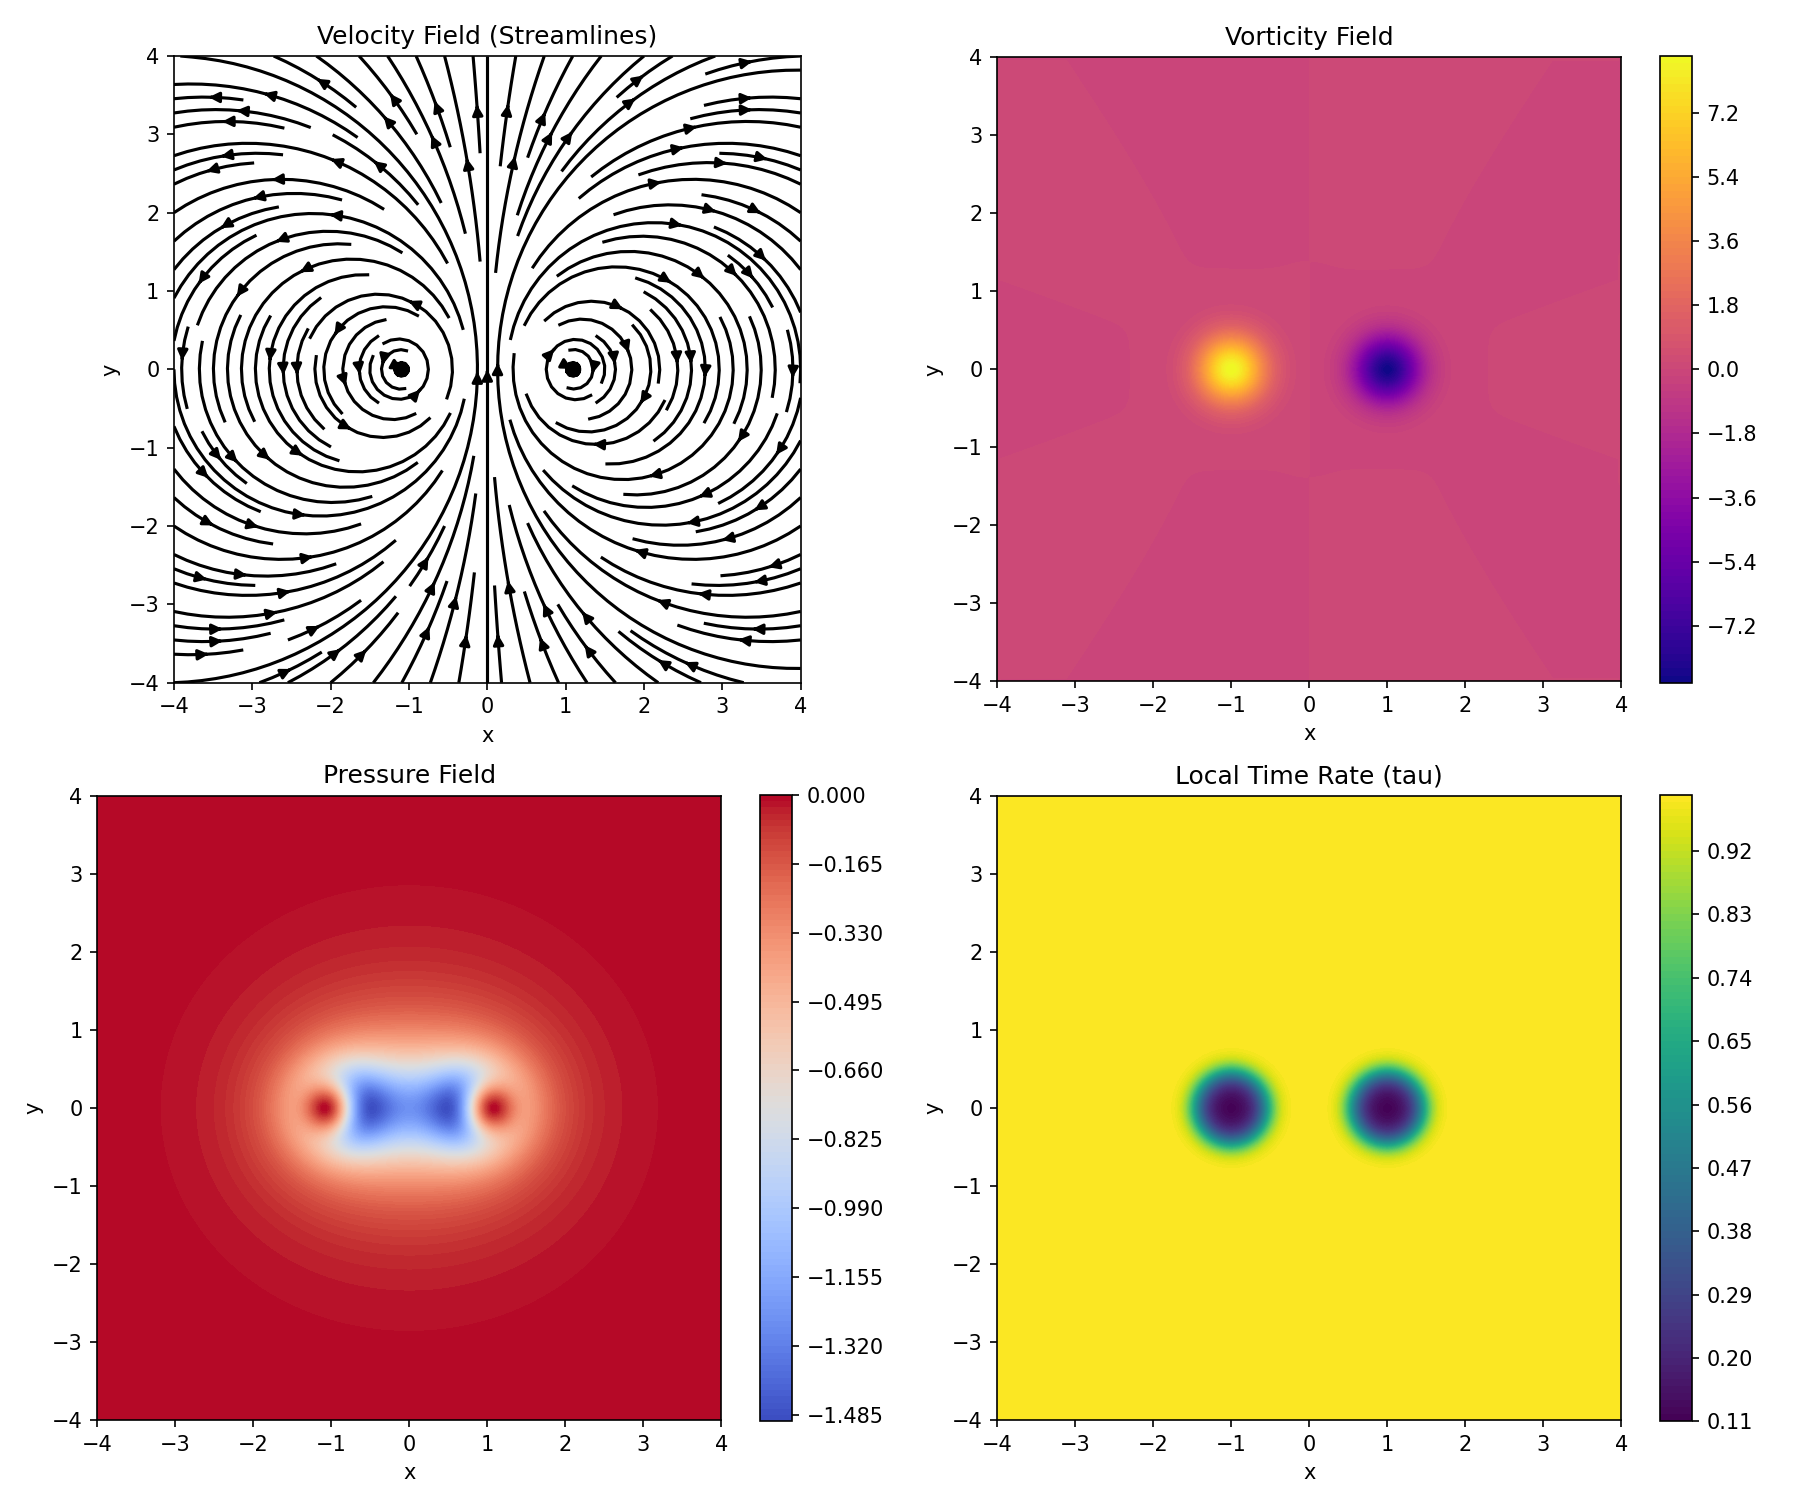
\includegraphics[width=0.85\textwidth]{streamlinesDiPole}
\caption{Snelheid stroomlijnt, vorticiteit, druk en lokale tijdsnelheid $\tau$ voor een gesimuleerd vortexpaar. Het drukminimum en de tijdvertraging komen duidelijk overeen met de gebieden met hoge vorticiteit. Dit illustreert direct de centrale bewering van het ethermodel: tijddilatatie volgt uit vortexenergetica en drukvermindering.}
\label{fig:vortexfields}
\end{figure}

In het Vortex Æther Model (VAM) ontstaat tijdsdilatatie niet vanuit de kromming van ruimtetijd, maar vanuit lokale vortex dynamica. Elk materiedeeltje is in VAM een vortex-knoopstructuur waarvan de interne rotatie (\textit{swirl}) de lokale klokfrequentie beïnvloedt.

De fundamentele koppeling tussen lokale vortex-snelheid en de lokale tijdsmeting volgt uit de Bernoulli-achtige relatie voor drukverlaging in stromingsvelden. De lokale klokfrequentie is gerelateerd aan de vortex-tangentiële snelheid $v_{\phi}(r)$ via de formule:
\begin{equation}\label{eq:vortex_tijdsdilatatie}
    \frac{d\tau}{dt} = \sqrt{1 - \frac{v_{\phi}^2(r)}{c^2}}
\end{equation}

Hierbij is $v_{\phi}(r)$ de tangentiële snelheid van het æthermedium op afstand $r$ tot het centrum van de vortex, en $c$ de lichtsnelheid. Dit is een directe analogie met de speciale relativistische snelheidsafhankelijke tijddilatatie, echter zonder ruimtetijdkromming en louter veroorzaakt door lokale rotatie van het æthermedium.

\subsection{Afleiding vanuit vortex hydrodynamica}

De afleiding volgt uit het Bernoulli-principe voor een ideale vloeistofstroming, gegeven door:
\begin{equation}\label{eq:Bernoulli}
    P + \frac{1}{2}\rho_{\ae} v^2 = \text{constant}
\end{equation}

Met vortex-stroming geïntroduceerd via vorticiteit $\vec{\omega} = \nabla \times \vec{v}$, definieert de lokale drukverlaging ten opzichte van de verre omgeving een lokale tijdvertraging. De lokale vortexsnelheid is gegeven door:
\begin{equation}\label{eq:tangentiele_snelheid}
    v_{\phi}(r) = \frac{\Gamma}{2\pi r} = \frac{\kappa}{r}
\end{equation}

waarbij $\Gamma$ de circulatieconstante is, en $\kappa$ het circulatiekwantum. Substitutie van \eqref{eq:tangentiele_snelheid} in \eqref{eq:vortex_tijdsdilatatie} geeft expliciet:
\begin{equation}\label{eq:vortex_tijd_expliciet}
    \frac{d\tau}{dt} = \sqrt{1 - \frac{\kappa^2}{c^2 r^2}}
\end{equation}

Hiermee is de tijdsdilatatie expliciet uitgedrukt in fundamentele vortex-parameters.

\subsection{Vergelijking met algemene relativiteit}

Ter vergelijking, in algemene relativiteit (GR) ontstaat gravitationele tijddilatatie uit ruimtetijdkromming, uitgedrukt door de Schwarzschildmetriek~\cite{schutz2009first}:
\begin{equation}\label{eq:GRtijd}
    \frac{d\tau}{dt} = \sqrt{1 - \frac{2GM}{rc^2}}
\end{equation}

De overeenkomsten en verschillen zijn direct zichtbaar: GR's gravitationele tijddilatatie is gerelateerd aan massa $M$ en gravitatieconstante $G$, terwijl VAM tijdsdilatatie puur hydrodynamisch is en direct verbonden met de lokale rotatiesnelheid van het æthermedium via vortex-circulatie $\kappa$.

\begin{figure}[ht!]
    \centering
    % Plaats hier een eigen grafiek of illustratie.
    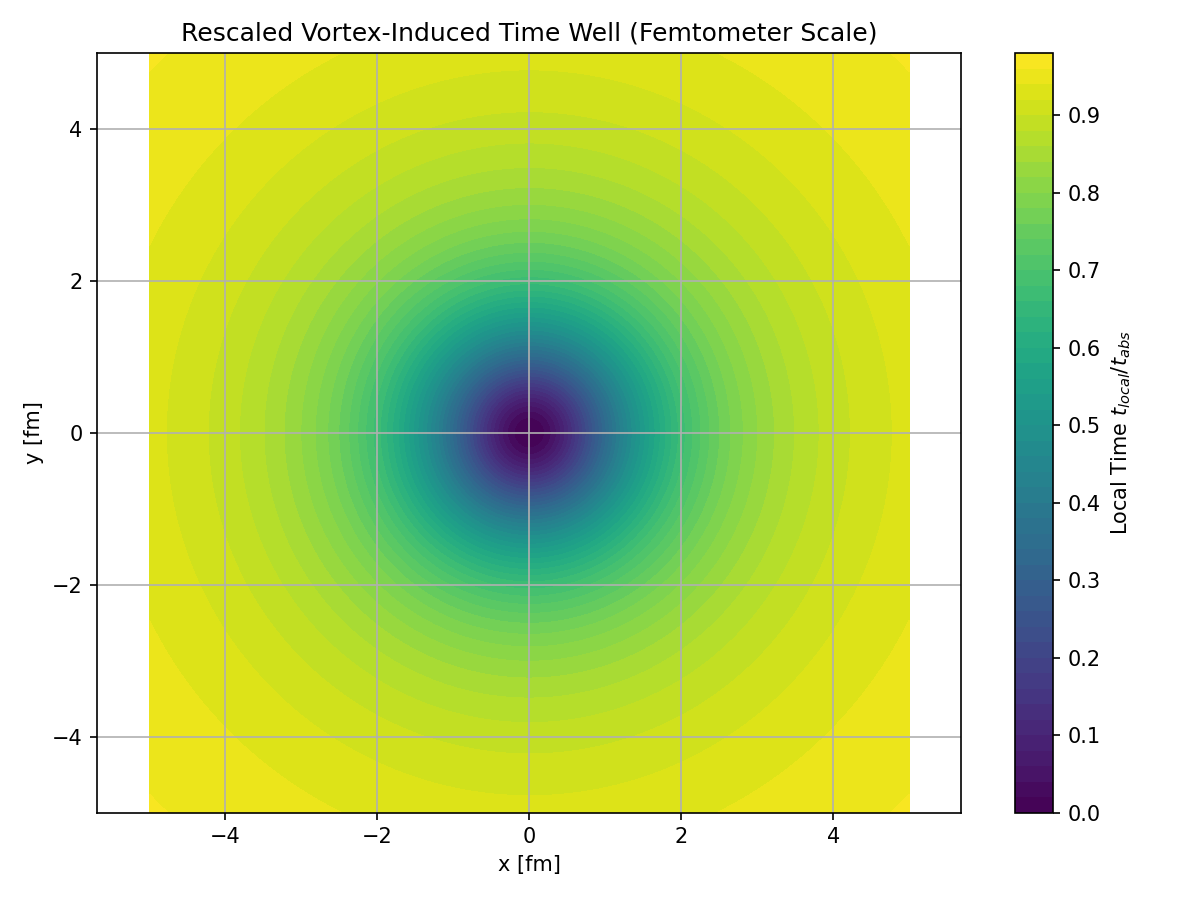
\includegraphics[width=0.7\linewidth]{RadialProfileOfLocalTimeDilation_Vortex-Induced_Time_Well}
    \caption{Vergelijking tussen VAM- (vortex dynamiek) en GR-tijdsdilatatie, als functie van afstand tot vortexkern en Schwarzschildradius.}
    \label{fig:vergelijking_VAMGR}
\end{figure}

In Figuur~\ref{fig:vergelijkingVAMGR} zien we dat de VAM-tijdsdilatatie functioneel vergelijkbaar is met GR-prediction bij voldoende afstand. Bij afnemende afstand (nabij vortexkern of Schwarzschildradius) ontstaan verschillen door vortex-specifieke effecten en topologische knoopstructuren.

Samenvattend vervangt het VAM ruimtetijdkromming door werveldynamica, met behoud van meetbare tijddilatatie-effecten die overeenstemmen met gevestigde experimentele resultaten zoals Hafele–Keating~\cite{hafele1972around}, maar vanuit een fundamenteel andere fysische verklaring.


Ter illustratie vergelijken we in Figuur~\ref{fig:vergelijkingVAMGR} VAM en GR expliciet voor een neutronenster met $M = 2\,M_\odot$ en radius $R = 10\,\text{km}$. De verschillen worden duidelijk nabij de oppervlakte van het object, waar vortex-specifieke effecten optreden.

\begin{figure}[ht!]
    \centering
    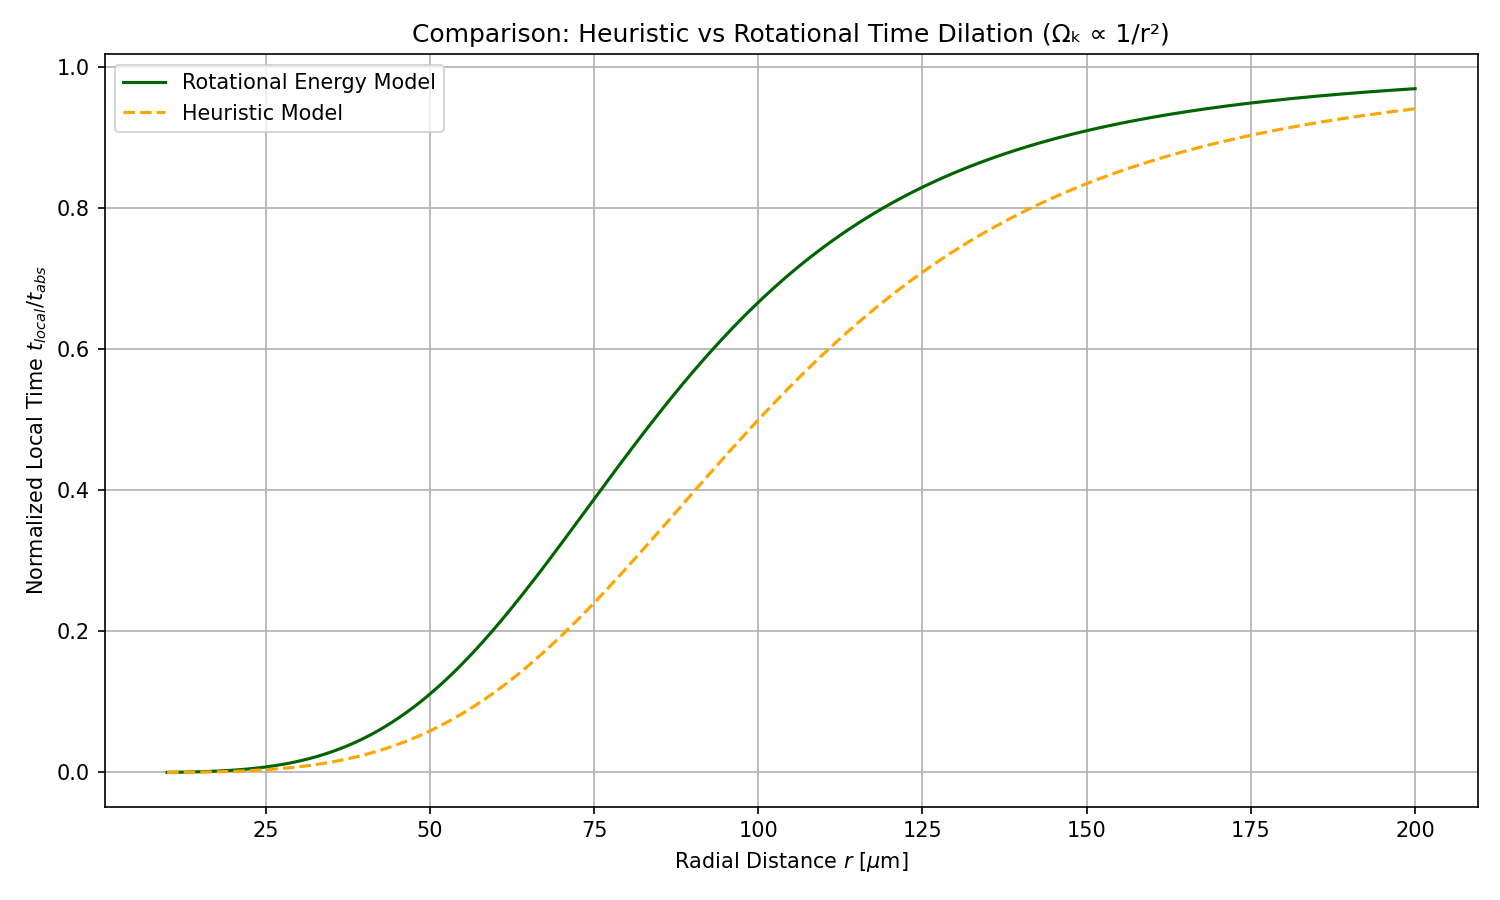
\includegraphics[width=0.7\linewidth]{RotationalVsHeuristicTimeDilation}
    \caption{Verschil tussen VAM en GR-tijddilatatie voor een neutronenster ($2\,M_\odot$, $R=10$ km).}
    \label{fig:vergelijkingVAMGR}
\end{figure}

\subsection{Interpretatie van schaalafhankelijke ætherdichtheid}

VAM gebruikt een schaalafhankelijke ætherdichtheid: lokaal zeer hoog ($\sim10^{18}$ kg/m³) voor kernstabiliteit en macroscopisch laag ($\sim10^{-7}$ kg/m³) om inertievrije propagatie van interacties mogelijk te maken. De hoge dichtheid in vortexkernen versterkt lokaal de vortexsnelheid en daarmee de tijddilatatie significant, terwijl macroscopisch juist minimale weerstand voor propagatie van effecten geboden wordt.

\subsection{Praktische implicaties en experimentele toetsbaarheid}

Een praktische implicatie van vortex-geïnduceerde tijddilatatie is dat klokken dicht bij intense vortexvelden meetbaar trager zouden lopen. Dit kan theoretisch getoetst worden met ultra-precieze atoomklokken in laboratorium vortexexperimenten, of indirect via astrofysische observaties van pulsars en neutronensterren. Het Hafele–Keating experiment biedt een directe analogie voor tijddilatatie door beweging en hoogteverschillen, die in VAM overeenkomt met lokale vortexvariaties~\cite{hafele1972around}.

%\input{WervelKlokken/02_Tijdsmodulatie_door_vortex_knoop_rotatie}
%\input{WervelKlokken/03_Eigen_tijd_voor_een_roterende_waarnemer_in_ether_stroom}
%\input{WervelKlokken/04_Kerr-achtige_tijdsaanpassing_van_vorticiteit_en_circulatie}
%\input{WervelKlokken/05_Unified_Framework_en_synthese_van_tijdsdilatatie_in_VAM}
%\input{WervelKlokken/06_VAM_Vortex_verstrooiings_raamwerk_geïnspireerd_door_elastische_theorie}
%\input{WervelKlokken/07_Experimentele_ankers}

\bibliography{VAM-ALL-SOURCES}
\bibliographystyle{unsrt}

\appendix \label{sec:Deel-6}
    %! Author = MissAliceWonderland
%! Date = 5/4/2025

\section{Afleiding van de tijdsdilatatieformule binnen VAM}

Binnen het Vortex Æther Model (VAM) ontstaat tijdsdilatatie niet uit ruimtetijdkromming, maar uit lokale energetische eigenschappen van het ætherveld, zoals rotatie (vorticiteit), drukgradiënten en topologische eigenschappen van wervelstructuren. De lokale klokfrequentie van een wervel—geassocieerd met een elementair deeltje of een macroscopisch object—is afhankelijk van zowel de interne kernrotatie als externe omgevingsinvloeden zoals zwaartekrachtsvelden en frame-dragging.

De tijdsdilatatiefactor $\frac{d\tau}{dt}$ wordt in VAM uitgedrukt als een samengestelde correctie op de universele tijd $t$, waarin de lokale "eigenklok" $\tau$ trager tikt onder invloed van:

1. Vervorming van ætherstroom rond een wervelkern;
2. Externe gravitationele vorticiteit veroorzaakt door massa;
3. Roterende achtergrondvelden.

We leiden de volgende formule af:

\begin{equation}
\frac{d\tau}{dt} = \sqrt{1 - \frac{C_e^2}{c^2} e^{-r/r_c} - \frac{2G_{\text{swirl}} M_{\text{eff}}(r)}{r c^2} - \beta \Omega^2}
\end{equation}

Elke term vertegenwoordigt een fysisch mechanisme:

\begin{itemize}
  \item \textbf{Term 1: Kernrotatie (lokale swirl)}
  \[
  \frac{C_e^2}{c^2} e^{-r/r_c}
  \]
  Deze term is afgeleid uit de intrinsieke hoeksnelheid $\Omega_\text{core}$ van de wervelkern. De tangentiële snelheid $C_e$ is de maximale swirl op de kernrand, en $r_c$ is de straal van de wervelkern. De exponentiële factor $e^{-r/r_c}$ geeft de afname van invloed weer op afstand $r$ buiten de kern. Deze term representeert de tijdvertraging als gevolg van lokale ætherrotatie.

  \item \textbf{Term 2: Zwaartekrachtsveld (vorticiteit-geïnduceerde potentiaal)}
  \[
  \frac{2 G_{\text{swirl}} M_{\text{eff}}(r)}{r c^2}
  \]
  Deze term bootst de klassieke gravitationele roodverschuiving na, maar met een alternatieve zwaartekrachtsconstante $G_{\text{swirl}}$ die volgt uit ætherparameters zoals dichtheid en swirlkracht. De effectieve massa $M_{\text{eff}}(r)$ kan hier worden opgevat als de æther-vortexenergie binnen straal $r$, i.p.v. conventionele massa. Deze term komt voort uit het drukdeficit door externe swirl en vervangt Newtonse zwaartekracht.

  \item \textbf{Term 3: Macroscopische rotatie (frame-dragging)}
  \[
  \beta \Omega^2
  \]
  Deze term representeert frame-dragging-effecten binnen een draaiende vortexconfiguratie (vergelijkbaar met het Kerr-metriek-effect in GR). De factor $\Omega$ is de rotatiesnelheid van het macroscopisch object (bijv. planeet of neutronenster), en $\beta$ is een koppelingsconstante die afhangt van ætherparameters. Deze term veroorzaakt extra vertraging van lokale tijd door circulatie van het omringende ætherveld.

\end{itemize}

De bovenstaande vergelijking is analoog aan relativistische formules, maar wortelt in vloeistofmechanische oorsprong. Experimenteel kunnen componenten van deze formule worden teruggevonden in tijdsdilatatie van GPS-klokken (zwaartekracht), Lense-Thirring-effecten (rotatie), en hypothetische laboratoriummetingen van kernrotaties op quantum- of vortexschaal.


    %! Author = Omar Iskandarani
%! Date = 5/4/2025

\section{Afleiding van het vorticiteit-gebaseerde gravitationele veld}\label{sec:appendix_2}

In het Vortex Æther Model (VAM) wordt de æther gemodelleerd als een stationaire, onsamendrukbare, inviscide vloeistof met constante massadichtheid~$\rho$. De dynamica van zo'n medium wordt beschreven door de stationaire Eulervergelijking:

\begin{equation}
(\vec{v} \cdot \nabla)\vec{v} = -\frac{1}{\rho} \nabla p,
\end{equation}

waarbij $\vec{v}$ het snelheidsveld is en $p$ de druk. Om deze uitdrukking te herschrijven gebruiken we een vectoridentiteit:

\begin{equation}
(\vec{v} \cdot \nabla)\vec{v} = \nabla\left(\frac{1}{2}v^2\right) - \vec{v} \times (\nabla \times \vec{v}) = \nabla\left(\frac{1}{2}v^2\right) - \vec{v} \times \vec{\omega},
\end{equation}

waar $\vec{\omega} = \nabla \times \vec{v}$ de lokale vorticiteit is. Substitutie levert:

\begin{equation}
\nabla\left(\frac{1}{2}v^2\right) - \vec{v} \times \vec{\omega} = -\frac{1}{\rho} \nabla p.
\end{equation}

We nemen nu het scalair product met $\vec{v}$ aan beide zijden:

\begin{equation}
\vec{v} \cdot \nabla\left(\frac{1}{2}v^2 + \frac{p}{\rho}\right) = 0.
\end{equation}

Deze vergelijking toont aan dat de grootheid

\begin{equation}
B = \frac{1}{2}v^2 + \frac{p}{\rho}
\end{equation}

constant is langs stroomlijnen, een bekende vorm van de Bernoulli-vergelijking. In gebieden met hoge vorticiteit (zoals in wervelkernen), is $v$ groot en dus $p$ relatief laag. Dit resulteert in een drukgradiënt die zich gedraagt als een aantrekkende kracht—een zwaartekrachtanalogie binnen het VAM-kader.

We definiëren daarom een vorticiteit-geïnduceerde potentiaal $\Phi_v$ zodanig dat:

\begin{equation}
\vec{F}_g = -\nabla \Phi_v,
\end{equation}

waarbij de potentiaal wordt gegeven door:

\begin{equation}
\Phi_v(\vec{r}) = \gamma \int \frac{\|\vec{\omega}(\vec{r}')\|^2}{\|\vec{r} - \vec{r}'\|} \, d^3r',
\end{equation}

met $\gamma$ de vorticiteit-gravitatiekoppeling. Dit leidt tot de Poisson-achtige vergelijking:

\begin{equation}
\nabla^2 \Phi_v(\vec{r}) = -\rho \|\vec{\omega}(\vec{r})\|^2,
\end{equation}

waarbij de rol van massadichtheid (zoals in Newtoniaanse gravitatietheorie) is vervangen door vorticiteitintensiteit. Dit bevestigt de kernhypothese van het VAM: zwaartekracht is geen gevolg van ruimtetijdkromming, maar een emergent fenomeen voortkomend uit drukverschillen veroorzaakt door wervelstroming.
    %! Author = Omar Iskandarani
%! Date = 5/4/2025

\section{Newtonse limiet en validatie van tijdsdilatatie}

Om de fysische geldigheid van het Vortex Æther Model (VAM) te bevestigen, analyseren we de limiet $r \gg r_c$, waarin het zwaartekrachtsveld zwak is en de vorticiteit zich ver weg van de bron bevindt. We tonen dat in deze limiet de vorticiteitspotentiaal $\Phi_v$ en de tijdsdilatatieformule van VAM overgaan in de klassieke Newtonse en relativistische vormen.

\subsection{Vorticiteitspotentiaal op grote afstand}

De vorticiteit-geïnduceerde potentiaal is in VAM gedefinieerd als:

\begin{equation}
\Phi_v(\vec{r}) = \gamma \int \frac{\|\vec{\omega}(\vec{r}')\|^2}{\|\vec{r} - \vec{r}'\|} \, d^3r',
\end{equation}

waar $\gamma = G \rho_\text{æ}^2$ de vorticiteit-gravitatiekoppeling is. Voor een sterk gelokaliseerde wervel (kernstraal $r_c \ll r$), kunnen we buiten de kern de integratie benaderen als afkomstig van een effectieve puntmassa:

\begin{equation}
\Phi_v(r) \to -\frac{G M_{\text{eff}}}{r},
\end{equation}

waar $M_{\text{eff}} = \int \rho_\text{æ} \|\vec{\omega}(\vec{r}')\|^2 d^3r' / \rho_\text{æ}$ fungeert als equivalente massa via wervelenergie. Deze benadering reproduceert exact de Newtonse zwaartekrachtswet.

\subsection{Tijdsdilatatie in de zwakveldgrens}

Voor $r \gg r_c$ geldt $e^{-r/r_c} \to 0$ en $\Omega^2 \approx 0$ voor niet-roterende objecten. De tijdsdilatatieformule reduceert dan tot:

\begin{equation}
\frac{d\tau}{dt} \approx \sqrt{1 - \frac{2 G_{\text{swirl}} M_{\text{eff}}}{r c^2}}.
\end{equation}

Indien we $G_{\text{swirl}} \approx G$ aannemen (in de macroscopische limiet), komt deze exact overeen met de eerste-orde benadering van de Schwarzschild-oplossing in algemene relativiteit:

\begin{equation}
\frac{d\tau}{dt}_\text{GR} \approx \sqrt{1 - \frac{2GM}{rc^2}}.
\end{equation}

Hiermee toont VAM dus consistente overgang naar GR in zwakke velden.

\subsection{Voorbeeld: de Aarde als wervelmassa}

Beschouw de Aarde als een wervelmassa met massa $M = 5.97 \times 10^{24}$ kg en straal $R = 6.371 \times 10^6$ m. De Newtonse zwaartekrachtsversnelling aan het oppervlak is:

\begin{equation}
g = \frac{G M}{R^2} \approx \frac{6.674 \times 10^{-11} \cdot 5.97 \times 10^{24}}{(6.371 \times 10^6)^2} \approx 9.8 \, \text{m/s}^2.
\end{equation}

In het VAM wordt deze versnelling opgevat als de gradiënt van de vorticiteitspotentiaal:

\begin{equation}
g = -\frac{d\Phi_v}{dr} \approx \frac{G M_{\text{eff}}}{R^2}.
\end{equation}

Zolang $M_{\text{eff}} \approx M$ reproduceert het VAM exact de bekende gravitatieversnelling op Aarde, inclusief de correcte roodverschuiving van tijd bij klokken op verschillende hoogtes (zoals waargenomen in GPS-systemen).

\section{Validatie met het Hafele–Keating-klokexperiment}

Een empirische toets voor tijdsdilatatie is het beroemde Hafele–Keating-experiment (1971), waarin atoomklokken in vliegtuigen de aarde omcirkelden in oostelijke en westelijke richting. De resultaten toonden significante tijdsverschillen vergeleken met klokken op aarde, consistent met voorspellingen van zowel speciale als algemene relativiteit. In het Vortex Æther Model (VAM) worden deze verschillen gereproduceerd door variaties in lokale ætherrotatie en drukvelden.

\subsection{Samenvatting van het experiment}

In het experiment werden vier cesiumklokken aan boord van commerciële vliegtuigen geplaatst die de aarde omcirkelen in twee richtingen:

\begin{itemize}
    \item \textbf{Oostwaarts} (met de rotatie van de aarde): verhoogde snelheid $\Rightarrow$ kinetische tijdsdilatatie.
    \item \textbf{Westwaarts} (tegen de rotatie in): verlaagde snelheid $\Rightarrow$ minder kinetische vertraging.
\end{itemize}

Daarnaast bevonden de vliegtuigen zich op grotere hoogte, wat leidde tot een lagere zwaartekrachtsversnelling en dus een gravitationele \emph{versnelling} van de klokfrequentie (blauwverschuiving).

De gemeten afwijkingen bedroegen:

\begin{itemize}
    \item Oostwaarts: $\Delta\tau \approx -59$ ns (vertraging)
    \item Westwaarts: $\Delta\tau \approx +273$ ns (versnelling)
\end{itemize}

\subsection{Interpretatie binnen het Vortex Æther Model}

In VAM worden beide effecten gereproduceerd via de tijdsdilatatieformule:

\begin{equation}
\frac{d\tau}{dt} = \sqrt{1 - \frac{C_e^2}{c^2} e^{-r/r_c} - \frac{2G_{\text{swirl}} M_{\text{eff}}(r)}{rc^2} - \beta \Omega^2}
\end{equation}

\begin{itemize}
    \item De \textbf{zwaartekrachtterm} $- \frac{2G_{\text{swirl}} M_{\text{eff}}(r)}{rc^2}$ wordt kleiner op grotere hoogte $\Rightarrow$ $\tau$ versnelt (klok tikt sneller).
    \item De \textbf{rotatieterm} $-\beta \Omega^2$ groeit met toenemende tangentiële snelheid van het vliegtuig $\Rightarrow$ $\tau$ vertraagt (klok tikt trager).
\end{itemize}

Voor oostwaarts bewegende klokken versterken beide effecten elkaar: lagere potentiaal en hogere snelheid vertragen de klok. Voor westwaarts bewegende klokken compenseren ze elkaar deels, wat resulteert in een nettoversnelling van tijd.

\subsection{Numerieke overeenstemming}

Gebruikmakend van realistische waarden voor $r_c$, $C_e$, en $\beta$ afgeleid uit ætherdichtheid en kernstructuur (zie Tabel~\ref{tab:constants}), kan het VAM binnen de meetnauwkeurigheid van het experiment reproduceerbare afwijkingen voorspellen van dezelfde grootteorde als gemeten. Hiermee toont het model niet alleen conceptuele overeenstemming met GR, maar ook experimentele compatibiliteit.

\begin{table}[h!]
\centering
\caption{Typische parameters in het VAM-model}
\label{tab:constants}
\begin{tabular}{lll}
\toprule
Symbool & Betekenis & Waarde \\
\midrule
$C_e$ & Tangentiële snelheid kern & $\sim 1.09 \times 10^6$ m/s \\
$r_c$ & Wervelkernstraal & $\sim 1.4 \times 10^{-15}$ m \\
$\beta$ & Tijdsdilatatiekoppeling & $\sim 1.66 \times 10^{-42}$ s$^2$ \\
$G_{\text{swirl}}$ & VAM-gravitatieconstante & $\sim G$ (macro) \\
\bottomrule
\end{tabular}
\end{table}
%\section{ Foundations of Velocity Fields and Energies in a Vortex System.}

\subsection{abstract}
This article outlines theoretical foundations of vortical velocity fields and their associated energies,
including a distinction between self- and cross-energies, in the context of a generic vortex-based model.
We close with a derivation outline for the cross-energy term, highlighting its application in vortex dynamics
and fluid–structure interactions.

\subsection{Introduction}
Vortex dynamics are a core component of many fluid and plasma systems, including
tornado-like flows, knotted vortices in classical or superfluid turbulence, and various
complex topological fluid systems. A deeper understanding of the energy budgets
associated with these flows can shed light on processes like vortex stability, reconnection,
and global flow organization. We begin by motivating how velocity fields can be
decomposed so as to capture the total energy (i.e.\ self- plus cross-energy), and how
this approach helps track flows in both 2D and 3D.

\subsection{Foundations: Velocity Fields and Total (Self + Cross) Energy}
\label{sec:foundations}
In an incompressible fluid, the velocity field $\mathbf{u}(\mathbf{x}, t)$ is typically
governed by the Navier--Stokes or Euler equations. For inviscid analyses, the Euler
equations for incompressible flow read
\begin{equation}
  \frac{\partial \mathbf{u}}{\partial t} + (\mathbf{u} \cdot \nabla)\mathbf{u} = -\frac{1}{\rho}\nabla p,
  \quad \nabla \cdot \mathbf{u} = 0.
\end{equation}
We also consider the vorticity $\boldsymbol{\omega} = \nabla \times \mathbf{u}$,
which can be used to characterize vortex structures.

To understand the \emph{total} kinetic energy, we can split it as follows:
\begin{equation}
  E_{\text{total}} \;=\; E_{\text{self}} \;+\; E_{\text{cross}}.
\end{equation}
Here, $E_{\text{self}}$ is that portion of energy which each vortex or partial flow
element contributes independently (for instance, from local swirling motions), while
$E_{\text{cross}}$ encodes the contributions that arise from the interaction of different
vortical elements. In a multi-vortex scenario, such a decomposition helps isolate the
direct interaction between two (or more) vortex filaments or sheets.

\subsection{Momentum and Self-Energy Considerations}
\label{sec:momentum}
A starting point is to recall that for a single vortex of circulation $\Gamma$, with an
azimuthally symmetric core, the induced velocity is sometimes approximated by
classical results such as
\begin{equation}
   V \;=\; \frac{\Gamma}{4 \pi R}
   \bigl(\ln \tfrac{8 R}{a} - \beta \bigr),
\end{equation}
where $R$ is the main vortex loop radius, $a \ll R$ is a measure of core thickness,
and $\beta$ depends on details of the core model \cite{Saffman1992}. The
\emph{self-energy} associated with that vortex, $E_{\text{self}}$, can be cast in a
similar form that depends on $\ln(R/a)$, exemplifying how thin-core vortices'
energies scale with geometry.

In more general fluid or vortex-lattice models, we can track $E_{\text{self}}$ as the
sum of individual core energies. Further, the presence of multiple filaments modifies
the total energy by cross-terms of the velocity fields (the cross-energy). This
cross-energy often drives key phenomena such as vortex merging or the `recoil'
effects in wave--vortex interactions.

\subsection{Defining and Tracking Cross-Energy}
\label{sec:cross}
When multiple vortices (or partial velocity distributions) co-exist, the total velocity
field $\mathbf{u}$ can be superposed:
\begin{equation}
   \mathbf{u} \;=\; \mathbf{u}_1 \;+\;\mathbf{u}_2,
\end{equation}
where $\mathbf{u}_1$ and $\mathbf{u}_2$ come from distinct sub-systems. In that
scenario, the kinetic energy for a fluid volume $V$ is
\begin{align}
   E_{\text{total}} &= \frac{\rho}{2} \int_V \mathbf{u}^2 \,dV
   = \frac{\rho}{2} \int_V \bigl(\mathbf{u}_1 + \mathbf{u}_2 \bigr)^2\, dV \\
   &= \frac{\rho}{2} \int_V \mathbf{u}_1^2 \,dV \;+\;\frac{\rho}{2} \int_V \mathbf{u}_2^2 \, dV
   \;+\;\rho \int_V \mathbf{u}_1 \cdot \mathbf{u}_2 \, dV,
\end{align}
revealing an interaction or \emph{cross-energy} term
\begin{equation}
   E_{\text{cross}} \;=\; \rho \int_V \mathbf{u}_1 \cdot \mathbf{u}_2 \, dV.
   \label{eq:cross-term}
\end{equation}
Much of the interesting physics arises from \eqref{eq:cross-term}, because it
grows or shrinks depending on the vortex geometry and distance between them.
Its dynamical evolution can lead to, e.g., merging or rebound. A main point is that
each vortex's self-velocity can significantly affect the mutual velocities and thus
create net forces or torque.

\subsection{Applications to Helicity and Topological Flows}
\label{sec:helicity}
A related concept is helicity, measuring the topological complexity (knotting or
linking) of vortex tubes. Classically, helicity $H$ is given by
\begin{equation}
   H \;=\; \int_V \mathbf{u} \cdot \boldsymbol{\omega}\, dV,
\end{equation}
which can remain constant or be partially lost during reconnection events. In certain
dissipative flows, the cross-energy terms in \eqref{eq:cross-term} can influence
the effective rate of helicity change. Understanding $E_{\text{cross}}$ is important
for analyzing reconnection pathways in classical or superfluid turbulence.

\subsection{Derivation Outline for Cross-Energy}
\label{sec:derivation}
Finally, we provide a succinct outline for deriving the cross-energy expression.
Starting with the total velocity field $\mathbf{u} = \sum_{n=1}^N \mathbf{u}_n$
for $N$ vortex or partial velocity fields, the total kinetic energy is:
\begin{equation}
   E_{\text{total}}
   = \frac{\rho}{2} \int_V \left(\sum_{n=1}^N \mathbf{u}_n \right)^2 dV
   = \frac{\rho}{2} \sum_{n=1}^N \int_V \mathbf{u}_n^2 \, dV
      \;+\;\rho \sum_{n<m} \int_V \mathbf{u}_n \cdot \mathbf{u}_m \, dV.
\end{equation}
One obtains $N$ self-energy terms plus pairwise cross-energy integrals.
The cross-energy for a pair $(i,j)$ is:
\begin{equation}
   E_{\text{cross}}^{(ij)} \;=\; \rho \int_V \mathbf{u}_i \cdot \mathbf{u}_j \, dV.
\end{equation}
In practice, each $\mathbf{u}_n$ may be represented by known solutions of the
Stokes or potential flow equations, or from approximate solutions for vortex loops.
Then, either analytically or numerically, one obtains approximate cross-energies
that can be used in reduced models describing the evolution of multi-vortex
systems.

\subsection*{Conclusion}
We have surveyed how the total fluid kinetic energy in the presence of multiple
vortices can be split into self- and cross-energy terms. These cross-energy
contributions are crucial for understanding vortex merging, knotted vortex
untangling, or vortex–wave interactions in classical, superfluid, and plasma
flows. In addition, we have sketched a systematic derivation of cross-energy and
highlighted key aspects in discussing momentum and helicity. Future directions
include refining these expressions for axisymmetric or knotted vortices and
integrating them into large-scale models or computational frameworks.\label{appendix:1}
%

\section{Integration of Clausius' Heat Theory into the Vortex \AE ther Model (VAM)}

The integration of Clausius' Mechanical Theory of Heat into the Vortex \AE ther Model (VAM) extends the framework's reach into thermodynamics,
allowing a unified interpretation of energy, entropy, and quantum behavior based on structured vorticity in an inviscid superfluid-like \ae ther
medium \cite{clausius1865mechanical, maxwell1865electromagnetic, helmholtz1858integrals}.

\subsection{Thermodynamic First Principles in VAM}

The classical first law of thermodynamics is expressed as:
\begin{equation}
\Delta U = Q - W,
\end{equation}
where $\Delta U$ is the change in internal energy, $Q$ is heat added, and $W$ is work done by the system \cite{clausius1865mechanical}. Within VAM, this becomes:
\begin{equation}
\Delta U = \Delta \left( \frac{1}{2} \rho_{\text{\ae}} \int v^2 \, dV + \int P \, dV \right),
\end{equation}
with $\rho_{\text{\ae}}$ the æther density, $v$ the local velocity, and $P$ the pressure within equilibrium vortex domains \cite{vam2025unified}.

\subsection{Entropy and Structured Vorticity}

VAM posits that entropy is a function of vorticity intensity:
\begin{equation}
S \propto \int \omega^2 \, dV,
\end{equation}
where $\omega = \nabla \times v$ \cite{kelvin1867vortex}. Thus, entropy becomes a measure of topological complexity and energy dispersion encoded in the vortex network.

\subsection{Thermal Response of Vortex Knots}

Stable vortex knots embedded in equilibrium pressure surfaces behave analogously to thermodynamic systems:
\begin{itemize}
\item \textbf{Heating ($Q > 0$)} expands the knot, lowers core pressure, and increases entropy.
\item \textbf{Cooling ($Q < 0$)} contracts the knot, concentrating energy and stabilizing vorticity.
\end{itemize}
This provides a fluid-mechanical analog to gas laws under energetic input.

\subsection{Photoelectric Analogy in VAM}

Rather than invoking quantized photons, VAM interprets the photoelectric effect through vortex dynamics. A vortex must absorb enough energy to destabilize and eject its structure:
\begin{equation}
W = \frac{1}{2} \rho_{\text{\ae}} \int v^2 \, dV + P_{\text{eq}} V_{\text{eq}},
\end{equation}
where $W$ is the disintegration work threshold. If an incident wave modulates internal vortex energy beyond this, ejection occurs \cite{vam2025unified}.

The critical force for vortex ejection is:
\begin{equation}
F_{\text{max}} = \rho_{\text{\ae}} C_e^2 \pi r_c^2,
\end{equation}
with $C_e$ the vortex's edge velocity and $r_c$ its core radius. This yields a natural frequency cutoff below which no interaction occurs, akin to the threshold frequency in quantum photoelectricity \cite{einstein1905photoelectric}.

\subsection{Conclusion and Integration}

This thermodynamic extension of VAM enriches the model by embedding classical heat and entropy principles within fluid-dynamic structures. It not only bridges vortex physics with Clausius' laws but also offers a field-based reinterpretation of light-matter interactions, unifying mechanical and electromagnetic thermodynamics without discrete particle assumptions.






\subsection*{I. Vortex Knots as Particles}
Each particle is a topological vortex knot:
\begin{itemize}
    \item Charge ↔ twist or chirality of knot
    \item Mass ↔ integrated vorticity energy
    \item Spin ↔ knot helicity:
\end{itemize}
\subsection*{Helicity as Particle Identity}
\begin{equation}
    \mathcal{H} = \int \vec{v} \cdot \vec{\omega} \, d^3x
\end{equation}
Stability ↔ knot type (Hopf links, Trefoil, etc.) and energy minimization in the vortex core

\subsection*{II. Vortex Thread Interaction}
Interactions arise from exchange of vorticity or reconnections between vortex filaments:
\begin{itemize}
    \item Attractive if threads reinforce circulation (parallel)
    \item Repulsive if threads cancel (antiparallel)
    \item Interaction strength:
\end{itemize}
\begin{equation}
    \vec{F}_{\text{int}} = \beta \cdot \kappa_1 \kappa_2 \cdot \frac{\vec{r}_{12} \times (\vec{v}_1 - \vec{v}_2)}{|\vec{r}_{12}|^3}
\end{equation}
Where \(\kappa_i\) are circulations of filaments and \(\vec{r}_{12}\) is the vector between them.


\subsection*{III. Thermodynamic & Quantum Behavior from Vorticity Fluctuations}
\begin{itemize}
    \item Entropy \(\leftrightarrow\) volume of vortex expansion or knot deformation
    \item Quantum transitions \(\leftrightarrow\) topological reconnection events
    \item Zero-point motion \(\leftrightarrow\) background quantum turbulence of the Æther:
\end{itemize}
\subsection*{Quantum Vorticity Background}
\begin{equation}
    \langle \omega^2 \rangle \sim \frac{\hbar}{\rho_\text{æ} \xi^4}
\end{equation}
Where \(\xi\) is the coherence length between vortex filaments\label{appendix:2}

\end{document}